\documentclass[a4paper,12pt]{article}
\usepackage[left=2.5cm, right=2.5cm, top=3cm, bottom=3cm]{geometry}
\usepackage{amsmath, amsthm, amssymb}
\usepackage[spanish]{babel}
\usepackage{graphicx}
\usepackage[utf8]{inputenc}
\usepackage{amsmath}
\usepackage[dvipinamos]{xcolor}

\title{Proyecto Moogle}
\author{Ronald Provance Valladares C121} 
\date{Today}

\begin{document}
	\maketitle
\begin{figure}[h]
	\centering
	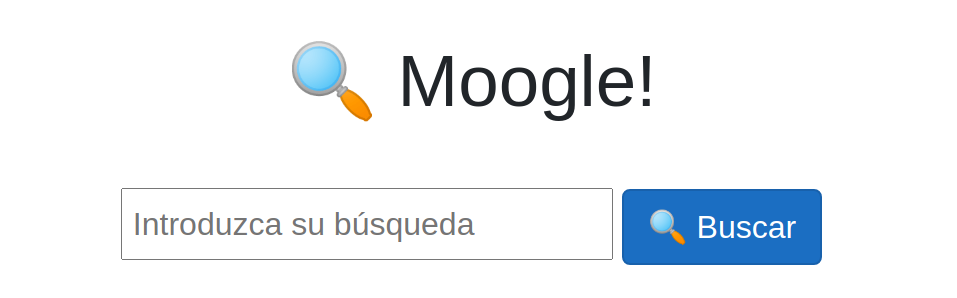
\includegraphics[width=17cm]{moogle.png}
\end{figure}


\begin{abstract}
	
	\begin{center}
		\large Todo lo básico que debe conocer para poder usar \textbf{Moogle!}:
	\end{center}

\begin{itemize}
	\item Moogle! es una aplicación que tiene como objetivo facilitar la búsqueda en un conjunto de documentos.

	\item Luego de implementar el motor de búsqueda he decidido redactar este informe con el propósito de explicar la realización del proyecto.
	
\end{itemize}
	Para llevar a cabo la tarea que se me ha asignado he utilizado lo que se conoce como modelo vectorial, que no es más que un modelo algebraico utilizado para el filtrado, indexado, recuperación y cálculo de relevancia de la información y además, mediante este modelo se pueden explotar las relaciones geométricas entre dos vectores documento (y términos) a fin de expresar las similitudes y diferencias entre términos.
\end{abstract}




\section{Funcionamiento}
Toda información solicitada será extraída de la colección de documentos (con extensión .txt) que se ingrese en la carpeta ‘Content’. \\
- El motor recibe una entrada por parte del usuario, llamado ‘query’, el cual puede contener algunos operadores que llegarían a optimizar la búsqueda, estos operadores son:\\

\renewcommand{\theenumi}{\Roman{enumi}}
\begin{enumerate}
	\item * este operador el usuario lo puede ingresar tantas veces como quiera antes de una palabra sin poner espacio, esto le dará mayor importancia o relevancia a los documentos que contengan esta palabra.
    \item ! el usuario debe colocarlo junto a la palabra, este negará (no devolverá) aquellos documentos que contengan esa palabra.\\
\end{enumerate}



\section{Clases}

A nivel estructural este proyecto cuenta con varias clases que van a tener determinadas funciones en la búsqueda de la información, estas son:


\subsection{La clase Implementation:}

	Esta clase va a tener la declaración de variables ‘generales’ y varios métodos:
	\renewcommand{\theenumi}{\arabic{enumi}}
	
	\begin{enumerate}
		
		\item Worktxt: en este método voy a operar sobre los documentos en la carpeta ‘Content’ para obtener su dirección y su título.\\
		\begin{figure}[h]
			\centering
			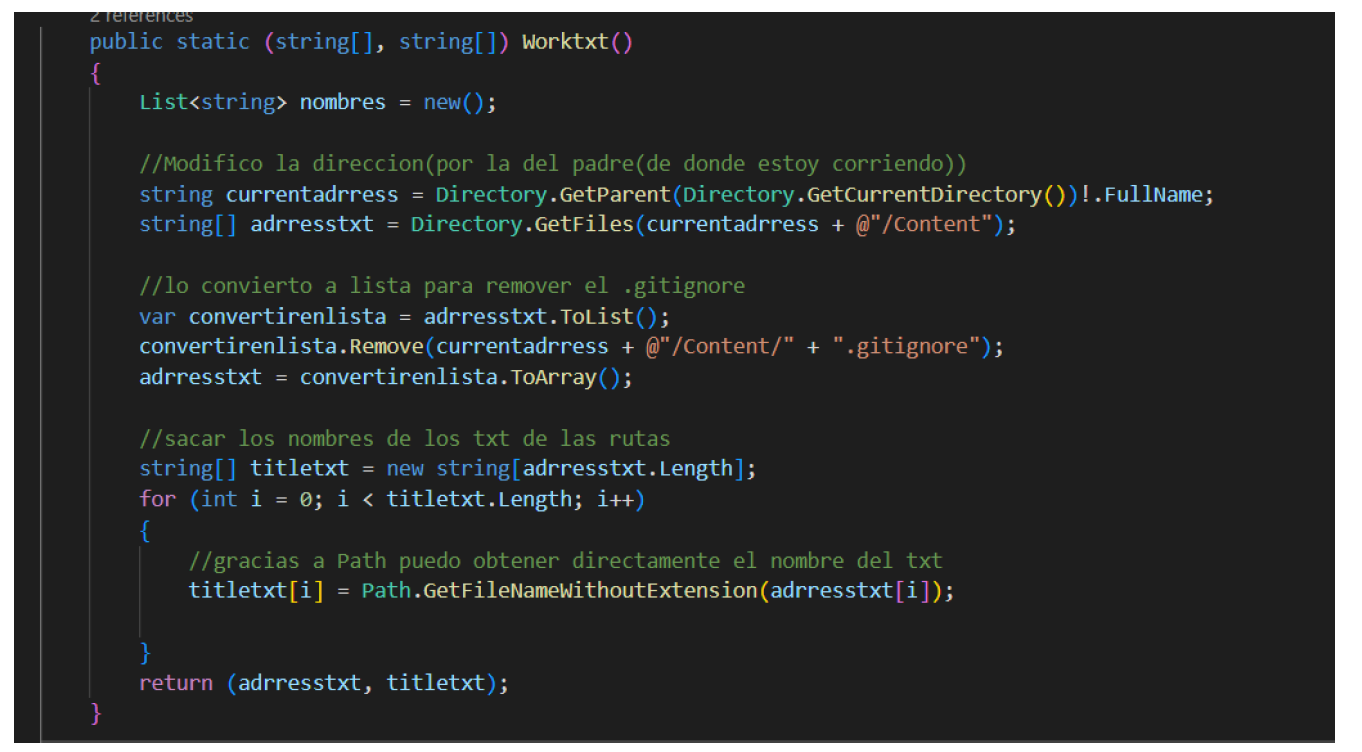
\includegraphics[width=13cm]{figura1.png}
			\caption{Método Worktxt}
		\end{figure}
		\newpage
		\item WorkWords: en este método voy a recorrer todos los documentos y voy a dejar solo las palabras y números (elimino los caracteres como ‘.’ y ‘,’ ) y guardo en un diccionario las palabras con su frecuencia y en listas guardo los documentos sin los caracteres y las palabras de todos los documentos sin repetir.\\
		\begin{figure}[h]
			\centering
			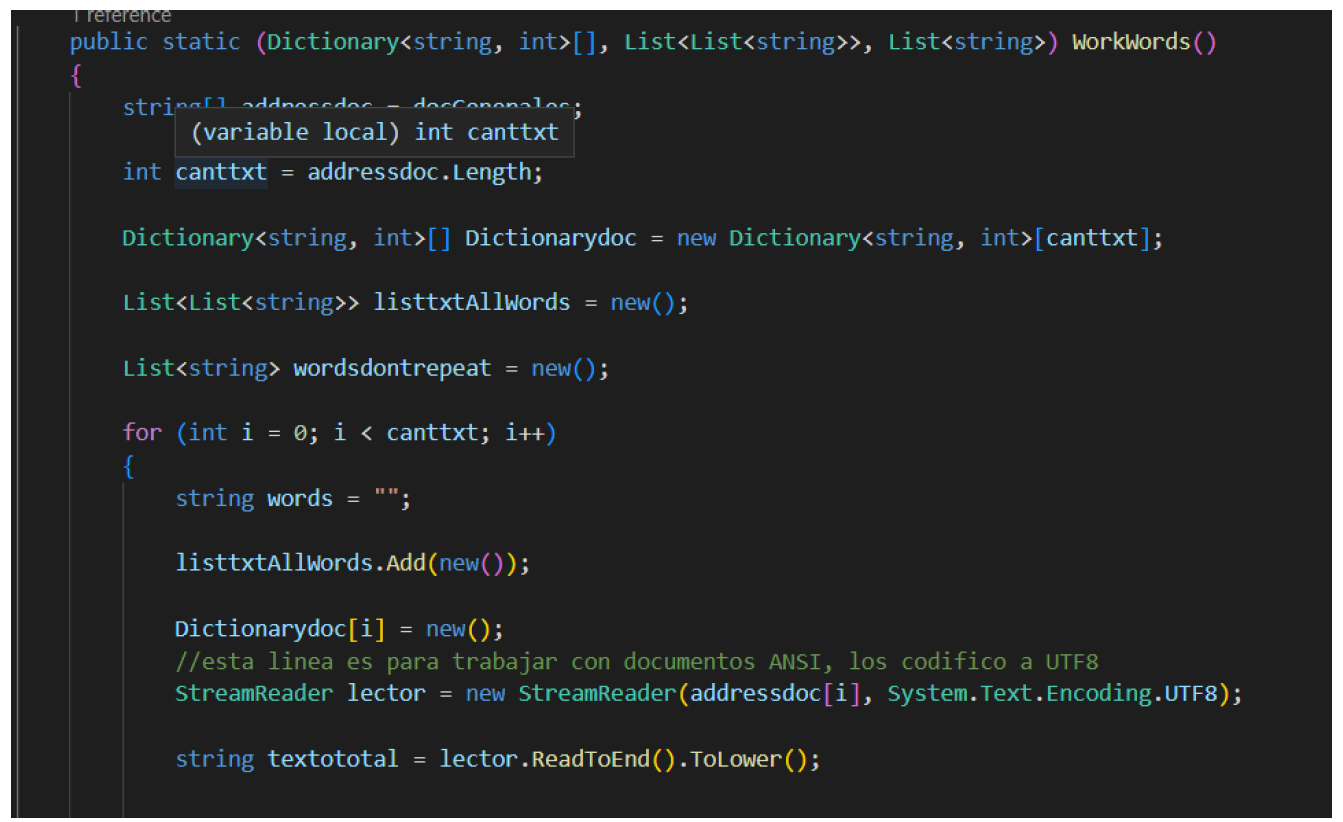
\includegraphics[width=13cm]{figura2.png}
			\caption{Método WorkWords}
		\end{figure}
		
		\item TFxIDF: en este método voy a calcular el TF-IDF de las palabras de los documentos, nótese en el código del calculo que le sumo una cantidad casi nula al contador, esto es una medida para impedir una indefinición dentro del cálculo que deriva en errores de búsqueda (aquí dejo una referencia, para más información, pude consultar las páginas de Wikipedia).\\
		
		$\ TF = \frac{FP}{N} $
		
		FP- Frecuencia de la palabra (Repetición)
		N- Número total de palabras.
		
		$\ IDF = \log\left(\frac{CD}{ND}\right) $
		
		CD- Cantidad total de TXT
		ND- Número de documentos que contiene la palabra
		
		
		TF-IDF (frecuencia de término – frecuencia inversa de documento): Es una medida numérica que expresa cuán importante es una palabra para un documento en una colección. Esta medida se utiliza a menudo como un factor de ponderación en la recuperación de información y la minería de texto. El TF-IDF aumenta proporcionalmente al número de veces que una palabra aparece en el documento, pero es compensada por la frecuencia de la palabra en la colección de documentos, lo que permite manejar el hecho de que algunas palabras son más frecuentes que otras.\\
		\newpage
		\begin{figure}[h]
			\centering
			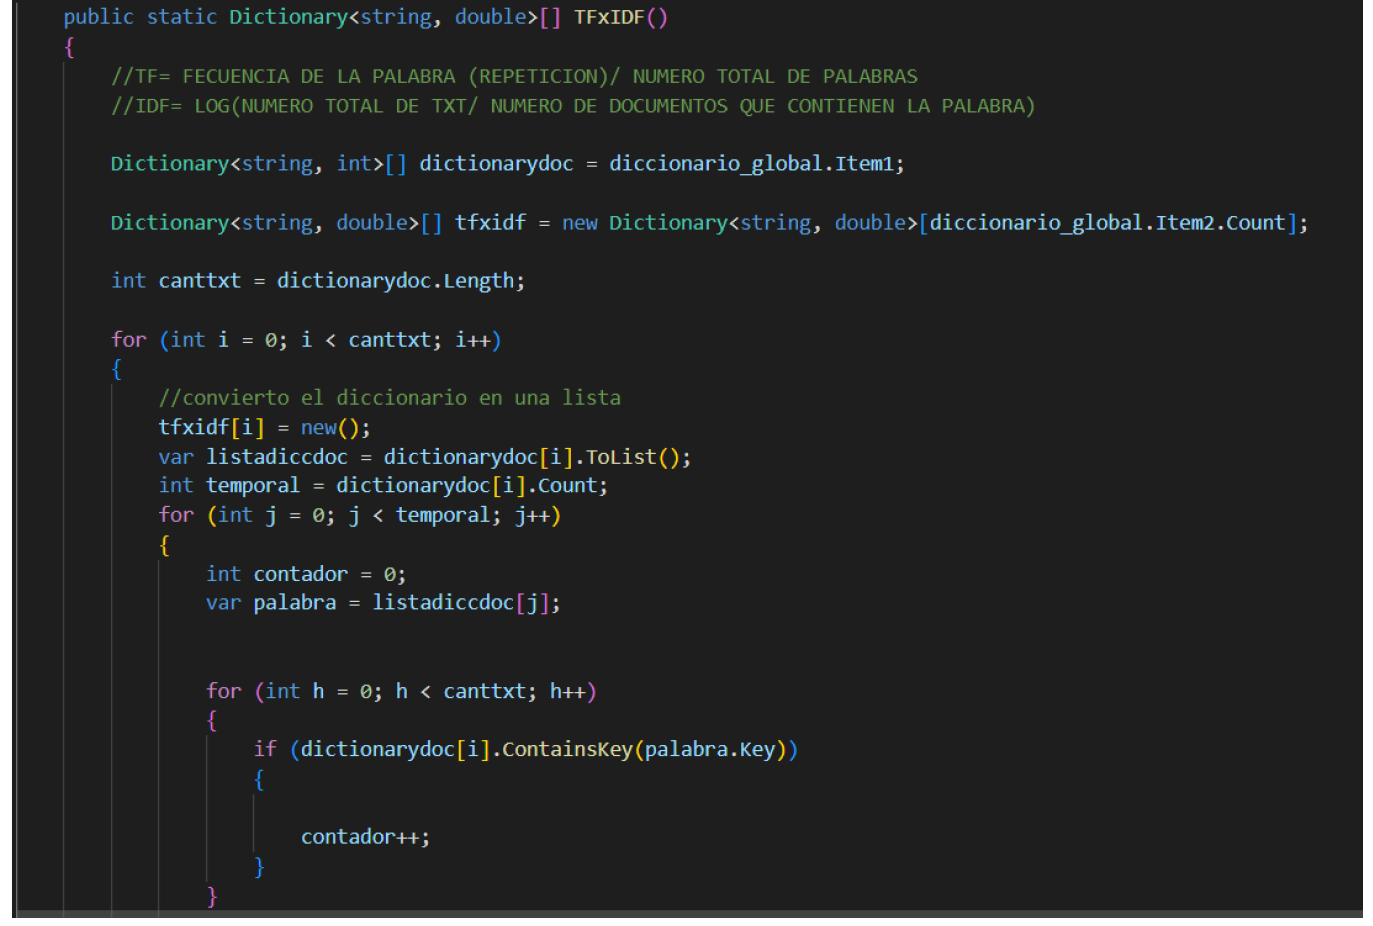
\includegraphics[width=13cm]{figura3.png}
			\caption{Método TFxIDF}
		\end{figure}
		
		\item QueryNormalizar: en este método voy a eliminar del query todo los caracteres que no sean letras o dígitos para posteriormente hacer su cálculo de TF-IDF, utilizando un método llamado TF e IDF de la query  del que voy a obtener un diccionario con las palabras y su valor de TF-IDF asociado.\\
		
		\begin{figure}[h]
			\centering
			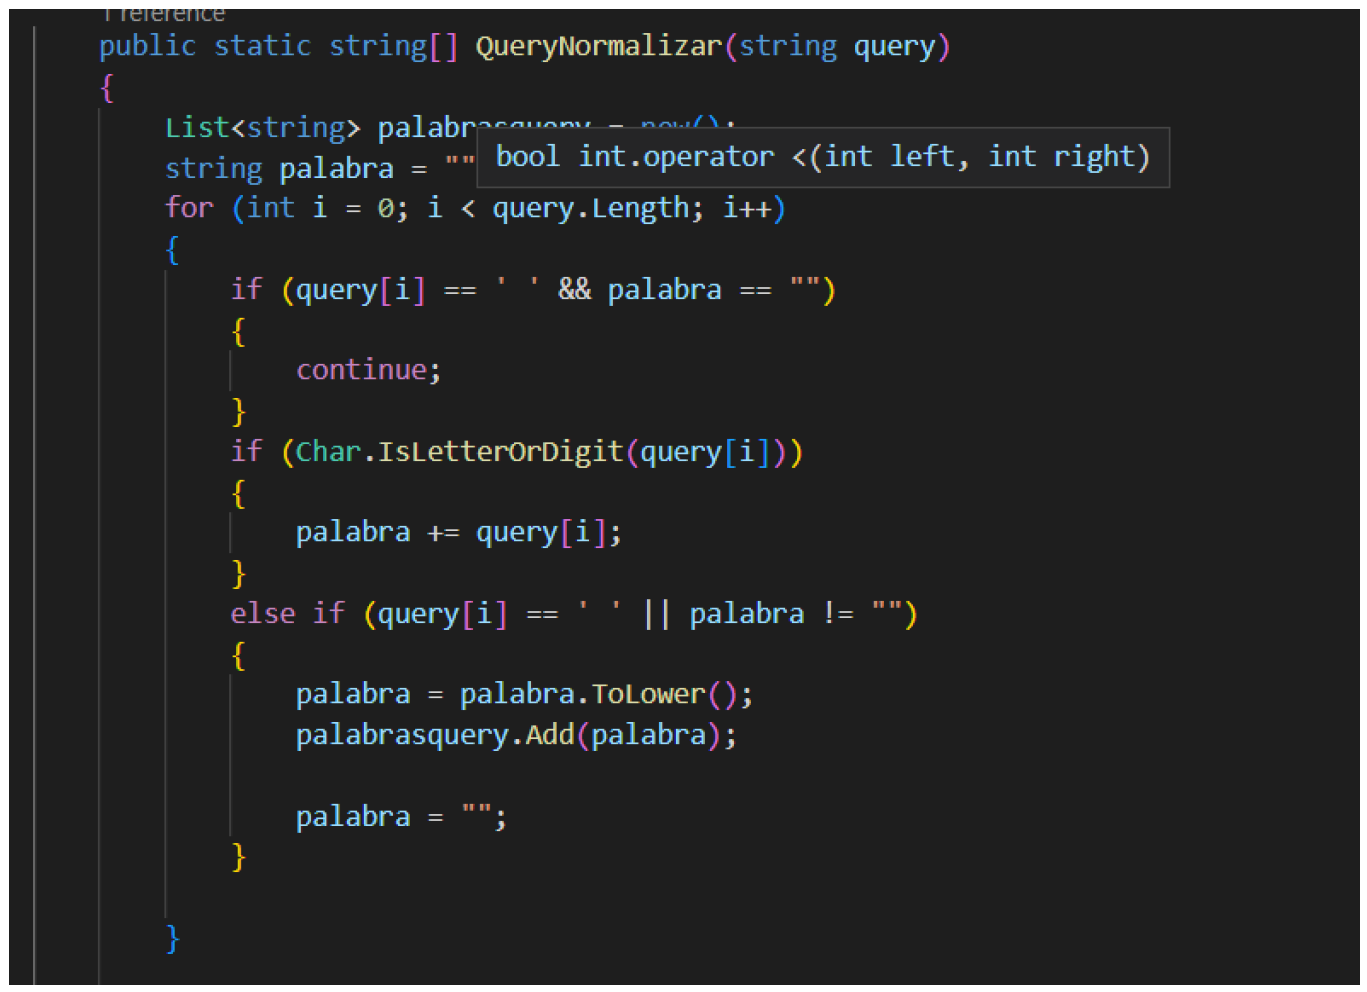
\includegraphics[width=13cm]{figura4.png}
			\caption{Método QueryNormalizar}
		\end{figure}
		
		\item QueryVectorizado: este método lo utilizo para guardar en un ‘array’ solo los valores de TF-IDF de las palabras del query. \\
		\begin{figure}[h]
			\centering
			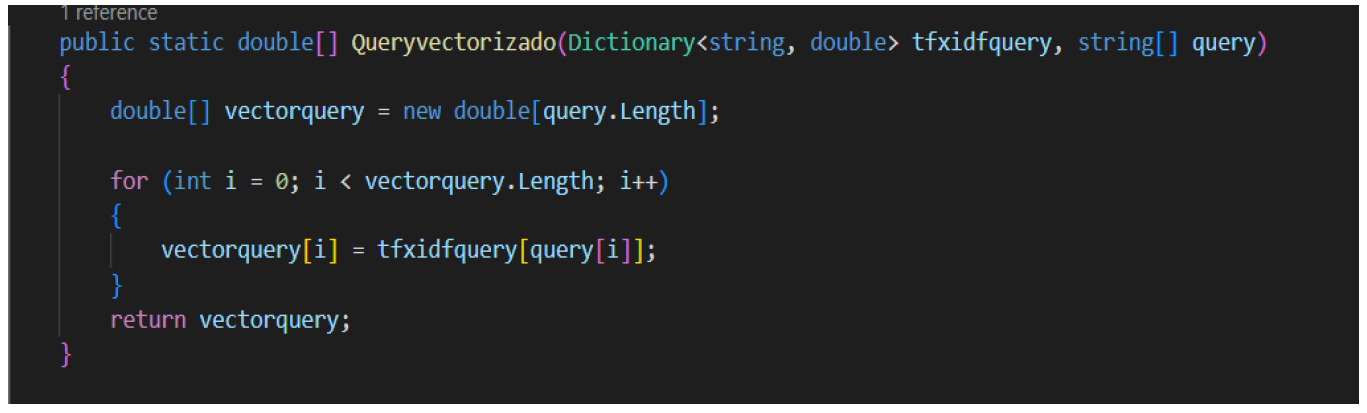
\includegraphics[width=13cm]{figura5.png}
			\caption{Método QueryVectorizado}
		\end{figure}
		
		\item Matriztfxidf: con este método voy a formar una matriz en la que voy a almacenar los valores de TF-IDF de las palabras del query en los documentos en los que aparezcan, si no aparecen les pongo valor 0.\\
		\begin{figure}[h]
			\centering
			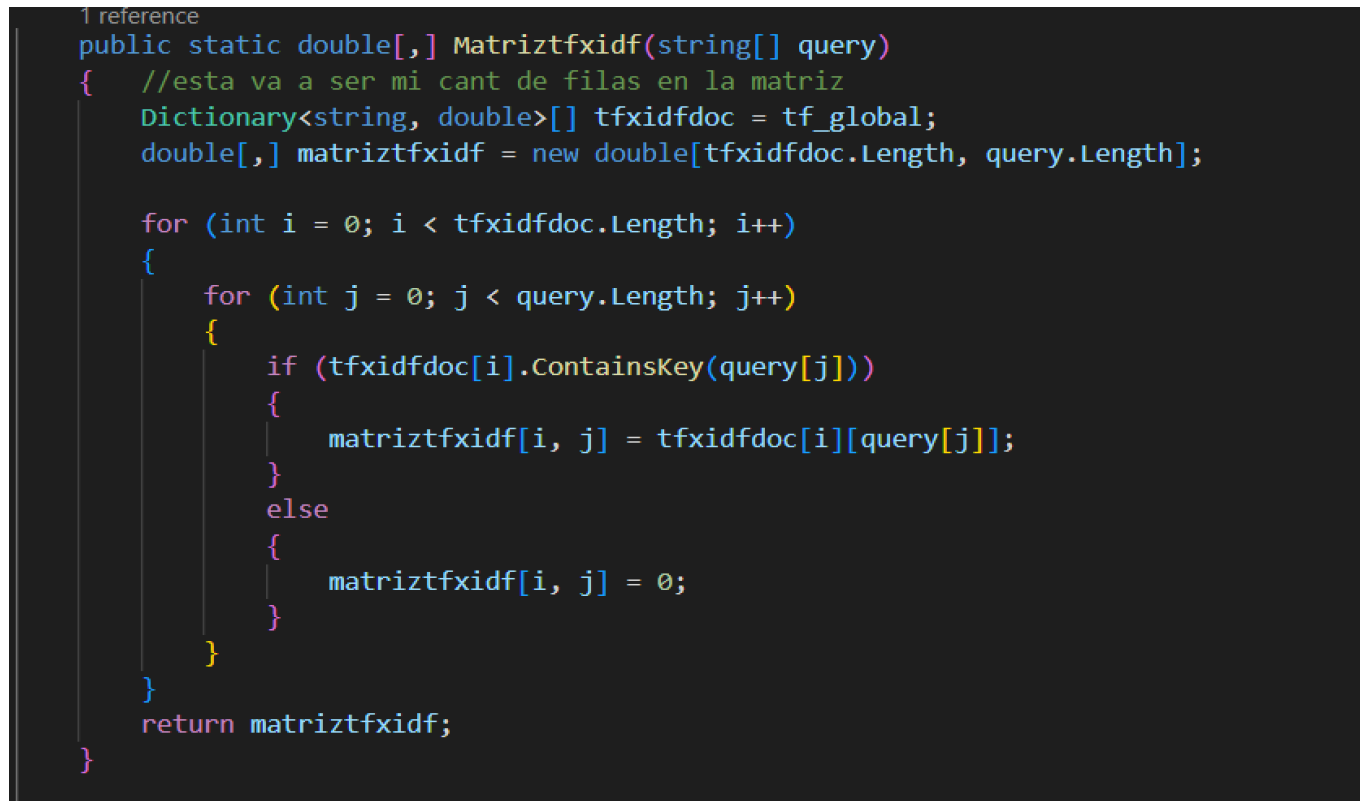
\includegraphics[width=13cm]{figura6.png}
			\caption{Método Matriztfxidf}
		\end{figure}
		
		\item SimilitudCos: en este método voy a calcular lo que se llama ‘similitud del coseno’ utilizando el query vectorizado y la matriz de TF-IDF antes calculados, y voy a obtener el ‘score’ de las palabras de los documentos con respecto al query ingresado, (dejo una referencia extraída de Wikipedia, para más información puede visitar la pagina oficial).\\
		Similitud del coseno: Es una medida de la similitud existente entre dos vectores e un espacio que posee un producto interior con el que se evalúa el valor del coseno del ángulo comprendido entre ellos. Esta función trigonométrica proporciona un valor igual a 1 si en ángulo comprendido es cero, es decir si ambos vectores apuntan a un mismo lugar. Cualquier ángulo existente entre los vectores, el coseno arrojaría un valor inferior a uno. Si los vectores fuesen ortogonales el coseno se anularía, y si apuntasen en sentido contrario su valor sería -1. De esta forma, el valor de esta métrica se encuentra entre -1 y 1, es decir en el intervalo cerrado [-1,1].\\
		\begin{figure}[h]
			\centering
			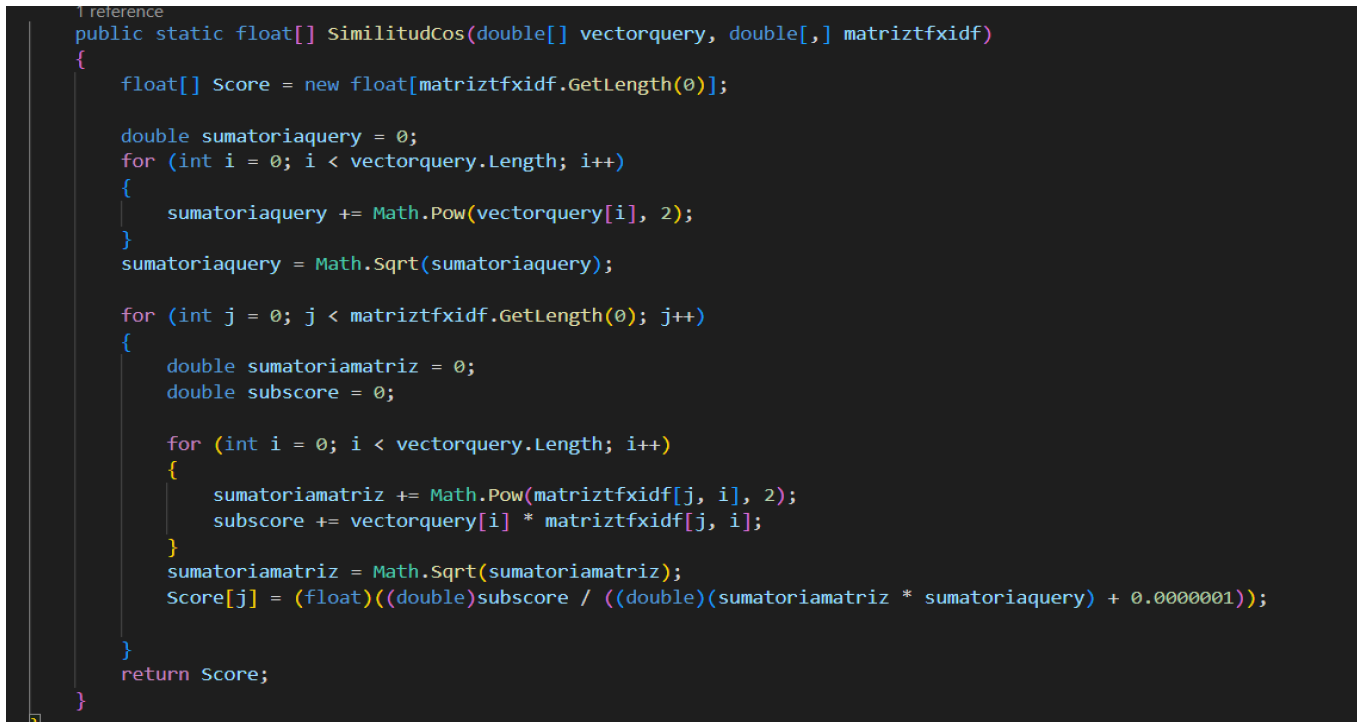
\includegraphics[width=13cm]{figura7.png}
			\caption{Método SimilitudCos}
		\end{figure}
		
	\end{enumerate}
	
	
	\subsection{La clase Levenshtein:}
	
	Esta clase es enteramente para la creación de las sugerencias del buscador a través del cálculo de distancias de Levenshtein, (debajo referencia extraída de Wikipedia).\\
	
	Levenshtein: Es el número mínimo de operaciones requeridas para transformar una cadena de caracteres en otra, se usa ampliamente en teoría de la información y ciencias de la computación. Se entiende por operación, bien una inserción, eliminación o la sustitución de un carácter. Este cálculo es muy útil para determinar cuan similares son dos cadenas de palabras y la empleo en mi proyecto con el fin de dar una sugerencia lo más acertada posible en caso de errores ortográficos en el query.\\
	
	Y aquí un pedazo de código de la clase que es el método calculo para calcular el porcentaje de cambio en la palabra
	\begin{figure}[h]
		\centering
		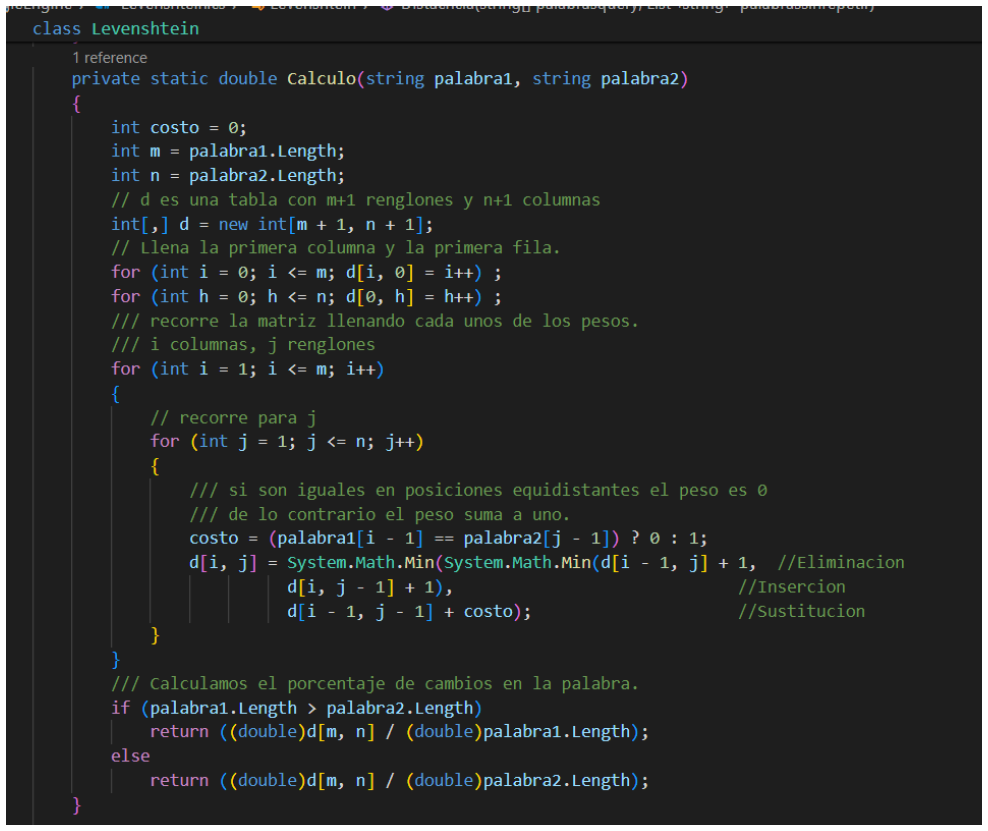
\includegraphics[width=14cm]{Levenshtein.png}
	\end{figure}


   \subsection{La clase Matriz}

    Aquí lleve las operaciones con matrices a la programación, ademas utilizo la multiplicación de matrices en el proyecto, ya que multiplico una matriz por un vector,que no es mas que una matriz de una sola columna (fila)\\
    
    \begin{figure}[h]
    	\centering
    	\includegraphics[width=14cm]{matrix.png}
    	\caption{Clase Matriz}
    \end{figure}
    
    
    \subsection{La clase Operadores:}
    
    En esta clase se encuentran los métodos con los que voy a definir la modificación sobre el ‘score’ en base a los operadores ingresados
    
    \renewcommand{\labelenumi}{$\bigstar$}
    \begin{enumerate}
    	
    \item En el caso del operador (!) uso el método ‘No Aparece’ los documentos que contengan a la palabra con este operador decidí, para que no aparezcan por ningún motivo, hacer su score 0, y de esta forma no presentarlo en los resultados de búsqueda.\\
    
    \begin{figure}[h]
    	\centering
    	\includegraphics[width=13cm]{operador1.png}
    	\caption{Operador "No Aparece"}
    \end{figure}
    
    \item En el caso del operador (*) uso el método ‘Asterisco’ decidí aumentar la relevancia de los documentos que contienen esa palabra al multiplicar el Score por la cantidad de (*) ingresados aumentado en 1.\\
    
    \begin{figure}[h]
    	\centering
    	\includegraphics[width=13cm]{operador2.png}
    	\caption{Operador "Asterisco"}
    \end{figure}
    
    \end{enumerate}
    
    
    \subsection{La clase Snippet:}
    
    En esta clase voy a tener un único método que será el encargado de construir un fragmento del documento donde se encuentren la(s) palabra(s) del query, este fragmento servirá como una breve introducción al contenido del documento.
    \begin{figure}[h]
    	\centering
    	\includegraphics[width=13cm]{snippet.png}
    	\caption{Clase Snippet}
    \end{figure}
    
    \subsection{La clase Moogle:}
    
    En esta clase se encuentran los llamados a las otras clases y métodos antes mencionados para hacer funcionar el buscador, además de un algoritmo de ordenación de los títulos de los documentos y el score para que sean devueltos en orden de mayor a menor score.\\
    
    Esta imagen muestra la llamada de métodos:\\
    \begin{figure}[h]
    	\centering
    	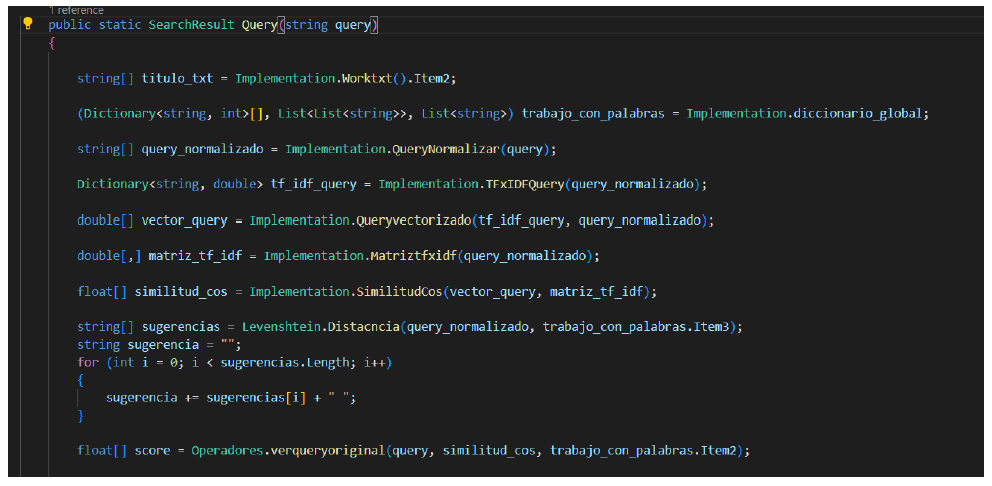
\includegraphics[width=14cm]{classmoogle.png}
    	\caption{Clase Moogle}
    \end{figure}



    \Large\textcolor{red}{A rasgos generales estas son las características de mi proyecto, espero lo disfrute.}
    \begin{center}
    \Huge\textcolor{red}{¡Muchas Gracias!}
    \end{center}
    
\end{document}
